\documentclass{article}
\usepackage[utf8]{inputenc}
\usepackage[russian]{babel}
\usepackage{graphicx}
\usepackage{caption}
\usepackage{float}
\usepackage{hyperref}
\usepackage{xcolor}
\usepackage[unicode, pdftex]{hyperref}
\usepackage[left=2cm,right=2cm,
    top=2cm,bottom=2cm,bindingoffset=0cm]{geometry}
    
\graphicspath{{pictures/}}
\DeclareGraphicsExtensions{.pdf,.png,.jpg}
\definecolor{urlcolor}{HTML}{003bed}
\hypersetup{pdfstartview=FitH, linkcolor=linkcolor,urlcolor=urlcolor, colorlinks=true}
\begin{document}
\begin{center}
\hfill \break

\LARGE{Математический анализ}\\
\hfill \break
\normalsize{Модуль 3\\
\hfill \break
2021 год\\
\hfill \break
«Интеграл функции одной переменной»}\\
\hfill \break
\hfill \break
\hfill \break
\hfill \break
\end{center}

\begin{flushright} Иванов Сергей, Иванов Алексей, Титов Даниил \end{flushright}
\begin{flushright} M3104 \end{flushright}
\vfill
\bigskip
\begin{center} Май 2021 \end{center}
\begin{center} ИТМО \end{center}
\thispagestyle{empty} % выключаем отображение номера для этой страницы
\newpage
\tableofcontents{}
\vfill
\bigskip
\begin{flushright} \href{https://www.overleaf.com/read/sbhfmhchwxzh}{Код отчёта на Overleaf (Latex)} \end{flushright}
\newpage
\section{Интегральная сумма}
\normalsize
\subsection{Исследуйте интегральную сумму функции $f(x)$, заданной на отрезке $[a, b]$}
\\
$ f(x) = \sin{x} $\\
$ [a, b] = [0; 3\pi/2] $\\
\subsubsection{Интегральная сумма}
\begin{figure}[h!]
\center{\fbox{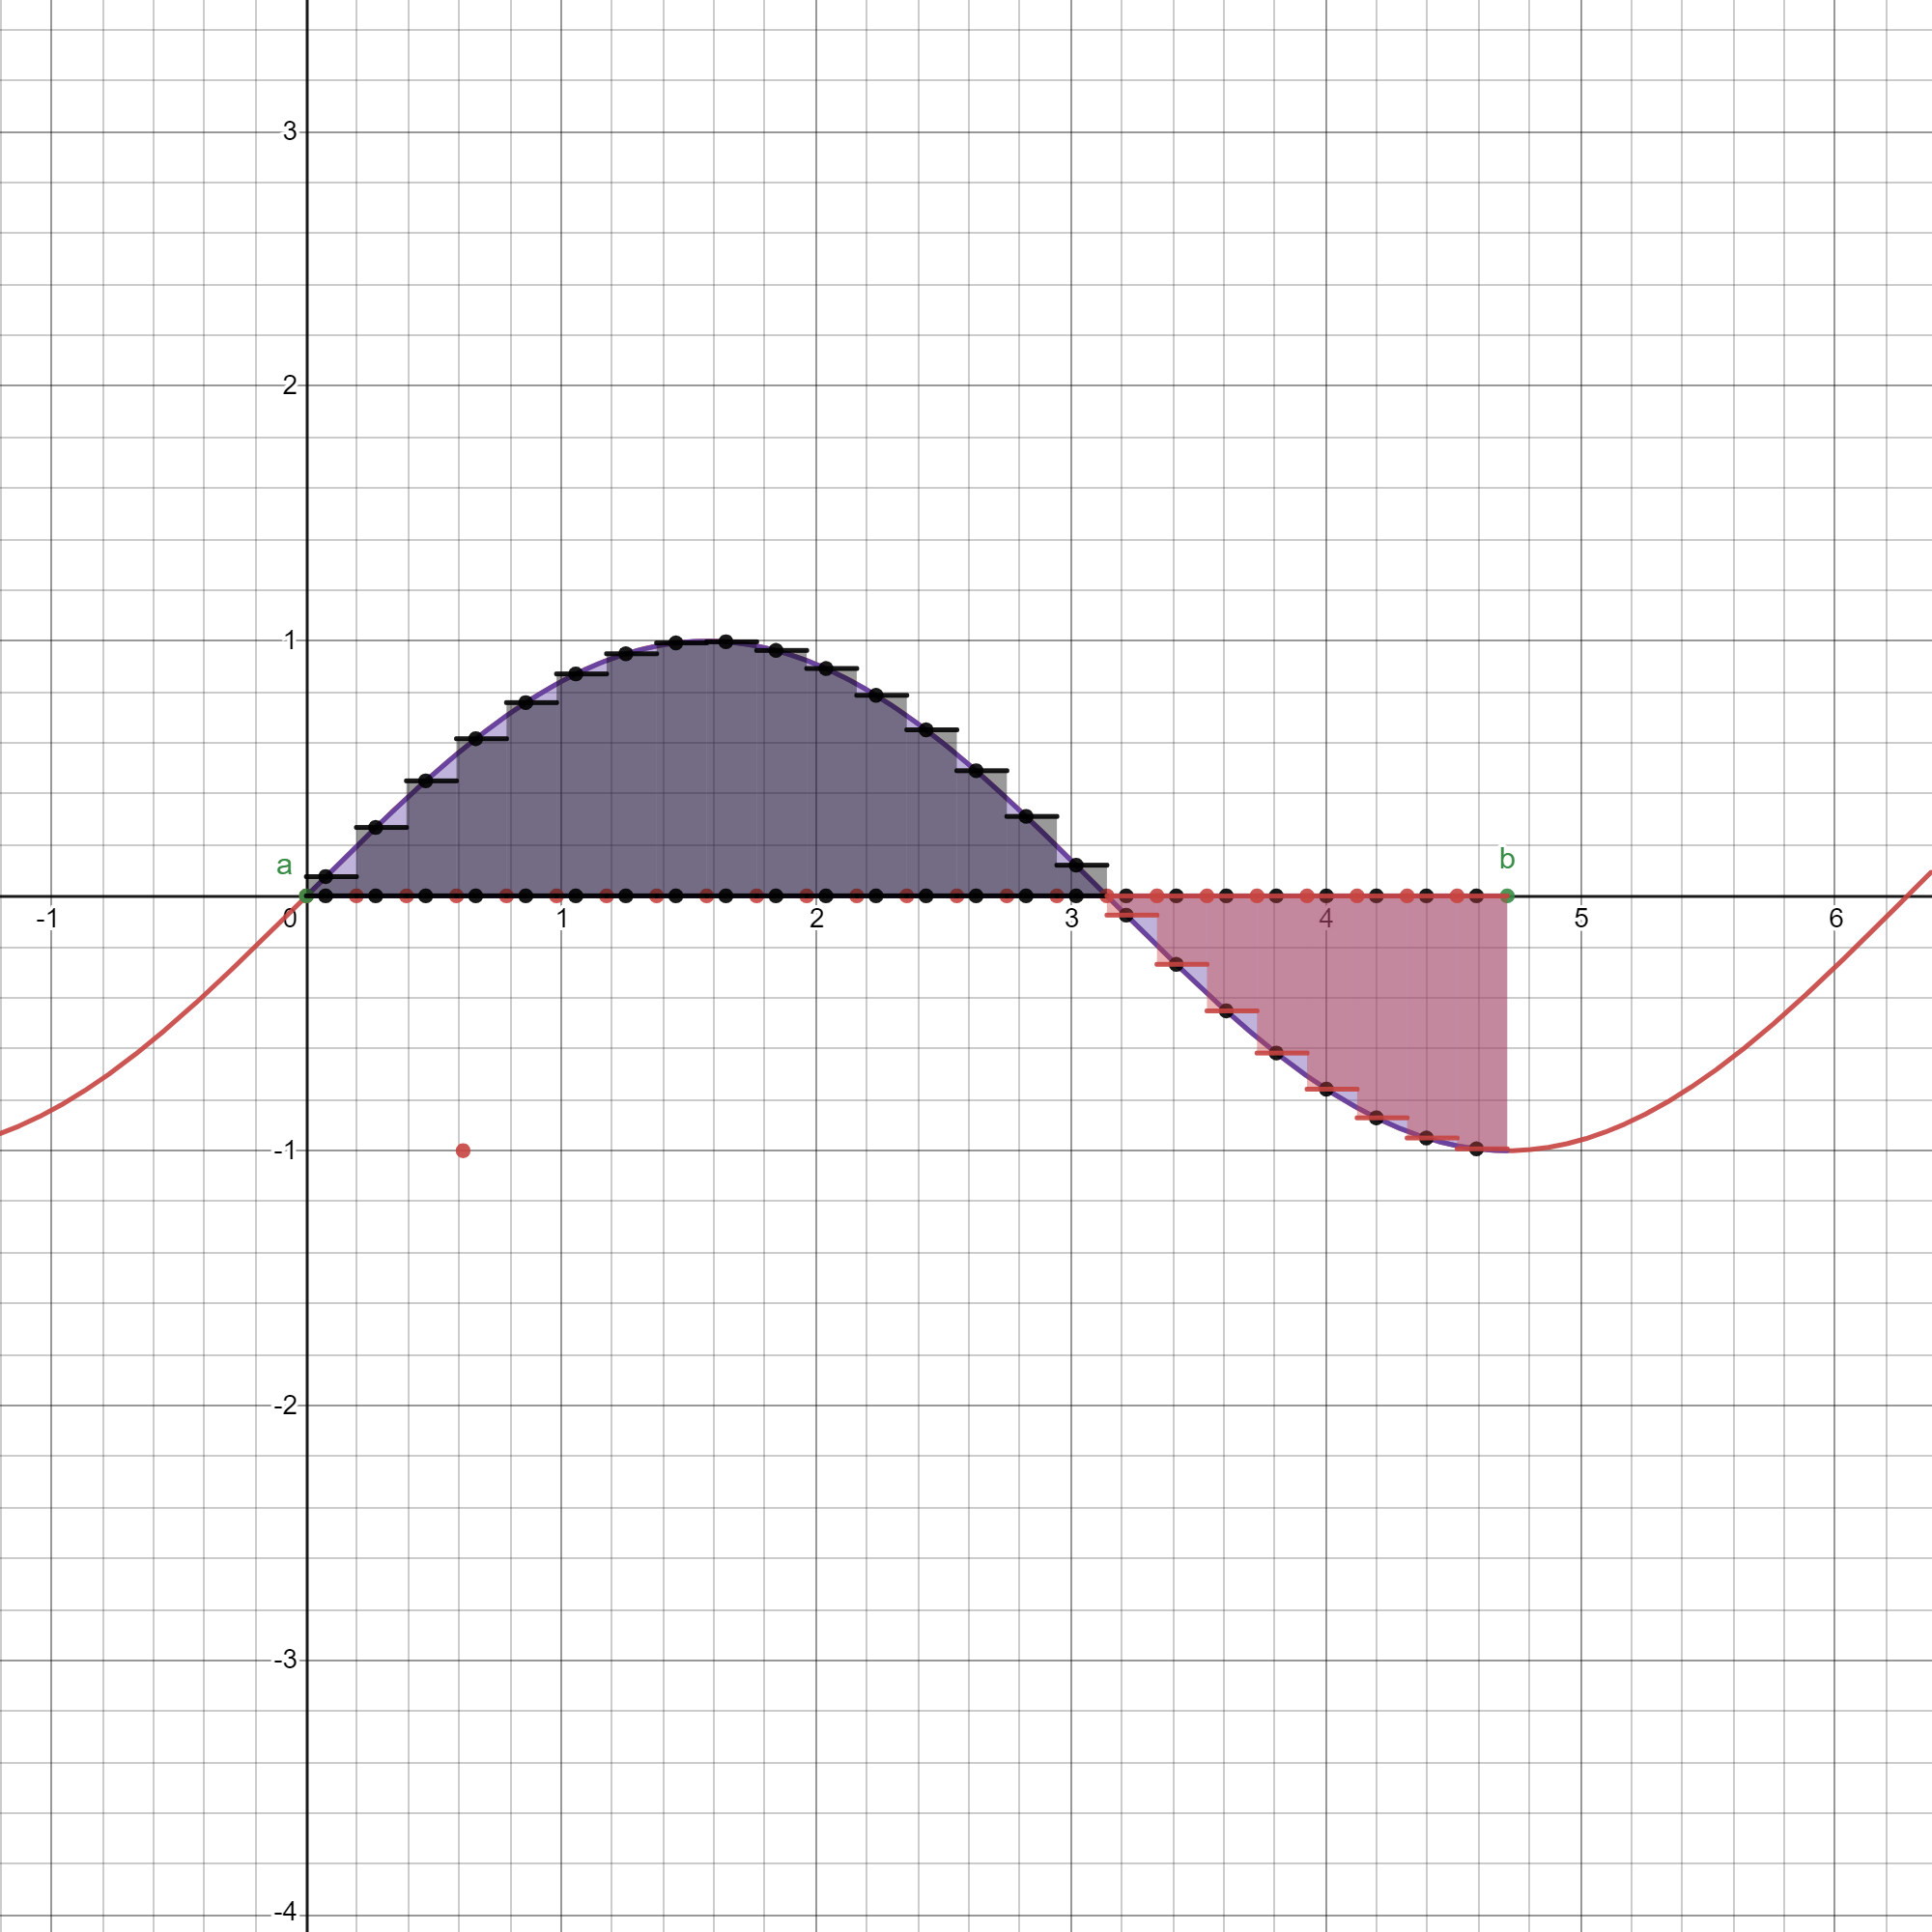
\includegraphics[scale=0.1]{1}}}
\caption*{\url{https://clck.ru/UjTMB}}
\end{figure}
\subsubsection{Последовательность интегральных сумм}

\begin{figure}[h!]
\center{\fbox{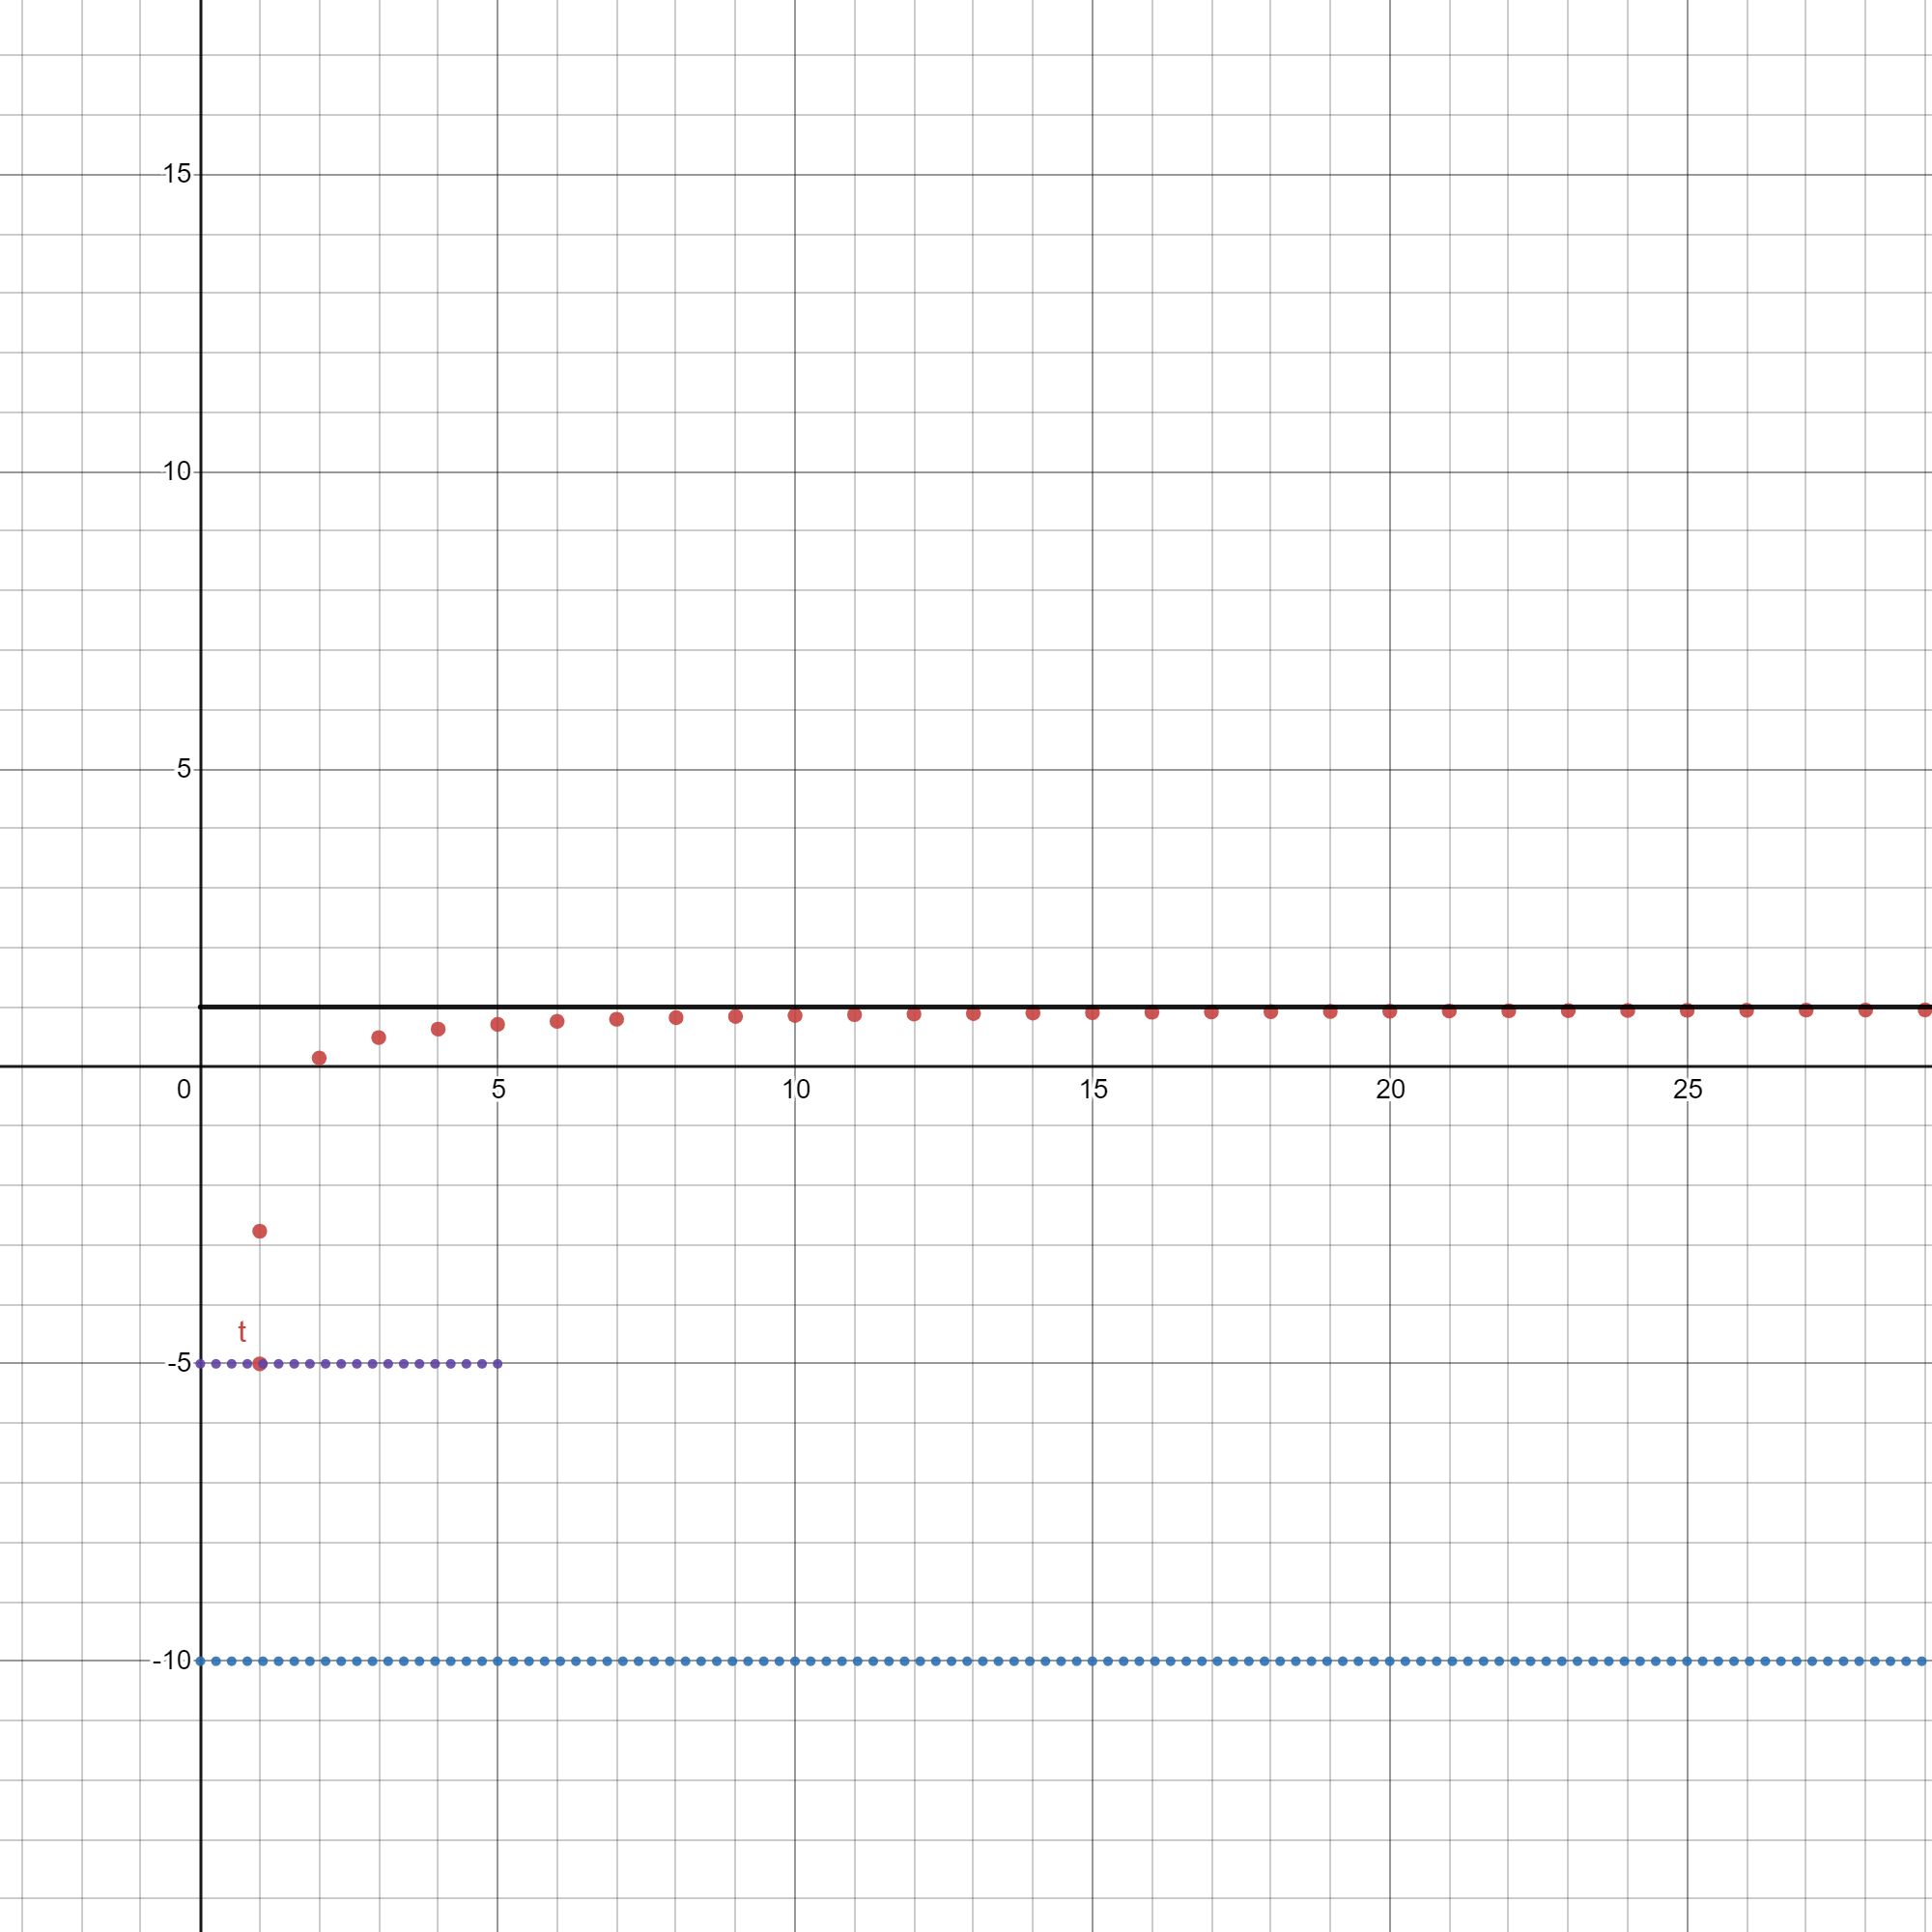
\includegraphics[scale=0.1]{12}}}
\caption*{\url{https://clck.ru/V6j8C}}
\end{figure}
\newpage
\\
\textbf{Примеры вычислений:}\\
$ h = \frac{b-a}{n} $\\
$ \sum\limits^{n}_{k = 1} f(a+(k-t)*h)*h $\\\\
$ t = 0 $:\\
1. $ n = 1 $: $ h = 4.71238898038 $, $ \sum\limits^{n}_{k = 1} = −4.71238898038 $\\
2. $ n = 10 $: $ h = 0.471238898038 $, $ \sum\limits^{n}_{k = 1} = 0.745806187809 $\\
3. $ n = 50 $: $ h = 0.0942477796077 $, $ \sum\limits^{n}_{k = 1} = 0.952135780258 $\\
$ t = 0.5 $:\\
1. $ n = 1 $: $ h = 4.71238898038 $, $ \sum\limits^{n}_{k = 1} = 3.33216220362 $\\
2. $ n = 10 $: $ h = 0.471238898038 $, $ \sum\limits^{n}_{k = 1} = 1.00931303637 $\\
3. $ n = 50 $: $ h = 0.0942477796077 $, $ \sum\limits^{n}_{k = 1} = 1.00037020607 $\\
$ t = 1 $:\\
1. $ n = 1 $: $ h = 4.71238898038 $, $ \sum\limits^{n}_{k = 1} = 0 $\\
2. $ n = 10 $: $ h = 0.471238898038 $, $ \sum\limits^{n}_{k = 1} = 1.21704508585 $\\
3. $ n = 50 $: $ h = 0.0942477796077 $, $ \sum\limits^{n}_{k = 1} = 1.04638355987 $\\
Все эти опыты можно повторить на нашем графике в desmos, и увидеть эти же результаты там.\\
\textbf{Вывод:}\\
С увеличением $ n $ увеличивается точность это можно заметить из примеров выше.
\newpage
\Large
\section{Несобственный интеграл}
\normalsize
\subsection{Исследуйте несобственный интеграл на сходимость при всех значениях параметра $ \alpha $}
\large $ \int\limits^{+\infty}_{1} \frac{\ln{x}}{x^{\alpha}}dx $\\
\normalsize
\subsubsection{Определите особую точку несобственного интеграла. Есть ли другие особые точки? К какому типу относится данный несобственный интеграл? Является ли подынтегральная функция неотрицательной на промежутке интегрирования?}
Подынтегральная функция является неотрицательной на промежутке интегрирования\\
Ещё особая точка: $ x = 0 $, но она не входит в предел интегрирования\\
$ D: x > 0 $\\
$ \lim\limits_{x\to 1^{+}} \frac{\ln{x}}{x^a} = \frac{0}{1} = 0 $\\\\
Тип интеграла:\\
1) Первого рода, так как пределы интегрирования от $ а $ до $ +\infty $\\
2) $ \int\limits^{+\infty}_{1} \frac{\ln{x}}{x^a}dx = \lim\limits_{A\to +\infty} \int\limits^A_1 \frac{\ln{x}}{x^a}dx $\\
$ a = 0 $\\
$ \lim\limits_{A\to +\infty} \int\limits^A_1 \ln{x}dx = \lim\limits_{A\to +\infty}(\ln{x}x - x |^A_1) = \lim\limits_{A \to +\infty} (A (\ln{A-1}) + 1) = \lim\limits_{A \to +\infty} (A (\ln{A - 1})) + \lim\limits_{A \to +\infty} (1) = \lim\limits_{A \to +\infty} (A) * \lim\limits_{A \to +\infty} (\ln{A - 1}) + 1 = +\infty $\\
Для некоторого $ a $:\\
$ \lim\limits_{A\to +\infty} (\frac{-\ln{x}}{(a-1)x^{(a-1)}} - \frac{1}{(a-1)^2 x^{a-1}} |^A_1) = \lim\limits_{A\to +\infty} (\frac{-\ln{A}}{(a-1)A^{a-1}} - \frac{1}{(a-1)^2 A^{a-1}} - (\frac{-\ln{1}}{(a-1)^2 * 1} - \frac{1}{(a-1)^2 * 1})) = \frac{1}{(a-1)^2} $\\
В зависимости от $ a $, может быть и сходящимся, и расходящимся
\subsubsection{Постройте графики подынтегральной функции при нескольких значениях параметра}
\begin{figure}[h!]
\center{\fbox{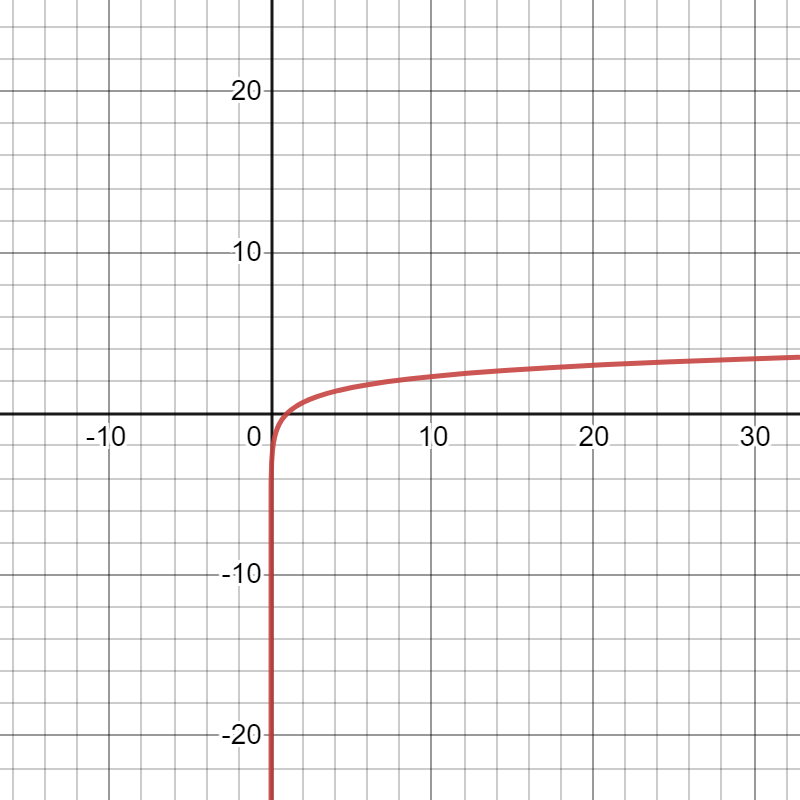
\includegraphics[scale=0.15]{20}}}
\caption*{$ \alpha = 0 $}
\end{figure}\\
\newpage
\begin{figure}[h!]
\center{\fbox{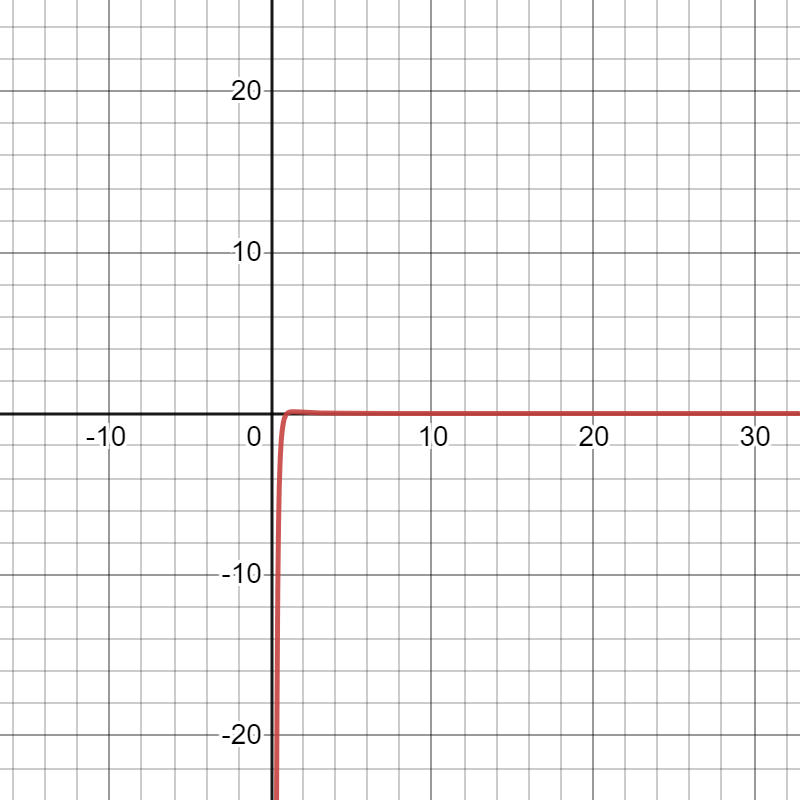
\includegraphics[scale=0.15]{23}}}
\caption*{$ \alpha = 3 $}
\end{figure}\\\\\\\\\\
\begin{figure}[h!]
\center{\fbox{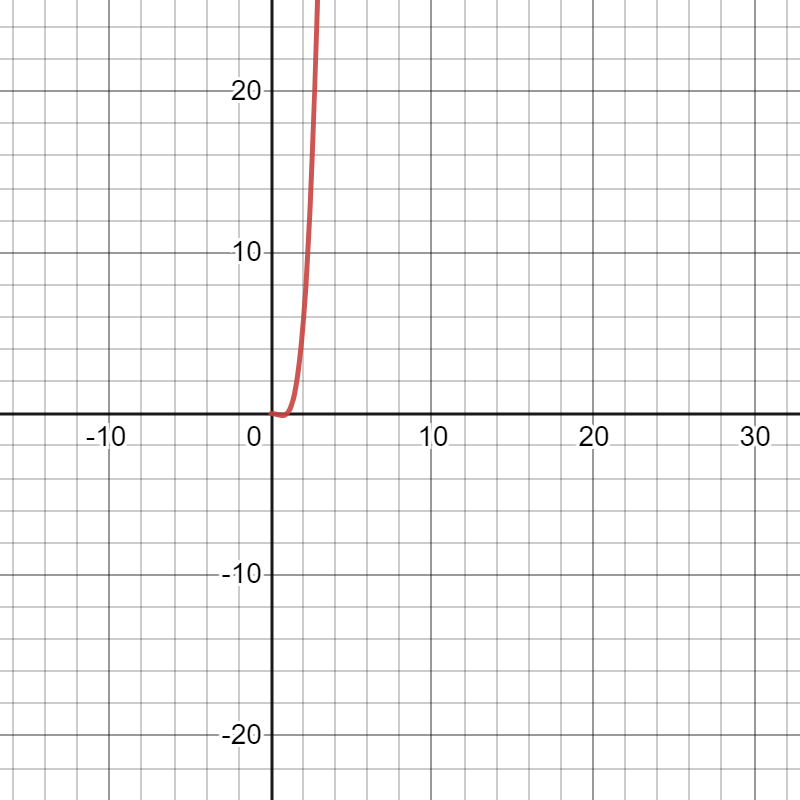
\includegraphics[scale=0.15]{2-3}}}
\caption*{$ \alpha = -3 $}
\end{figure}\\
\begin{figure}[h!]
\center{\fbox{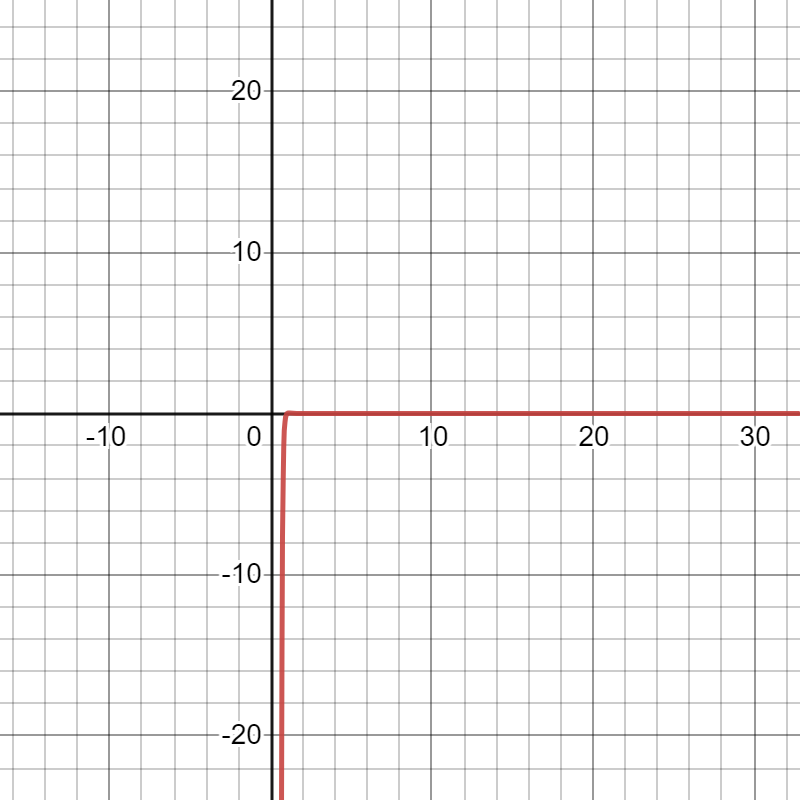
\includegraphics[scale=0.15]{210}}}
\caption*{$ \alpha = 10 $}
\end{figure}\\\\\\\\\\
\begin{figure}[h!]
\center{\fbox{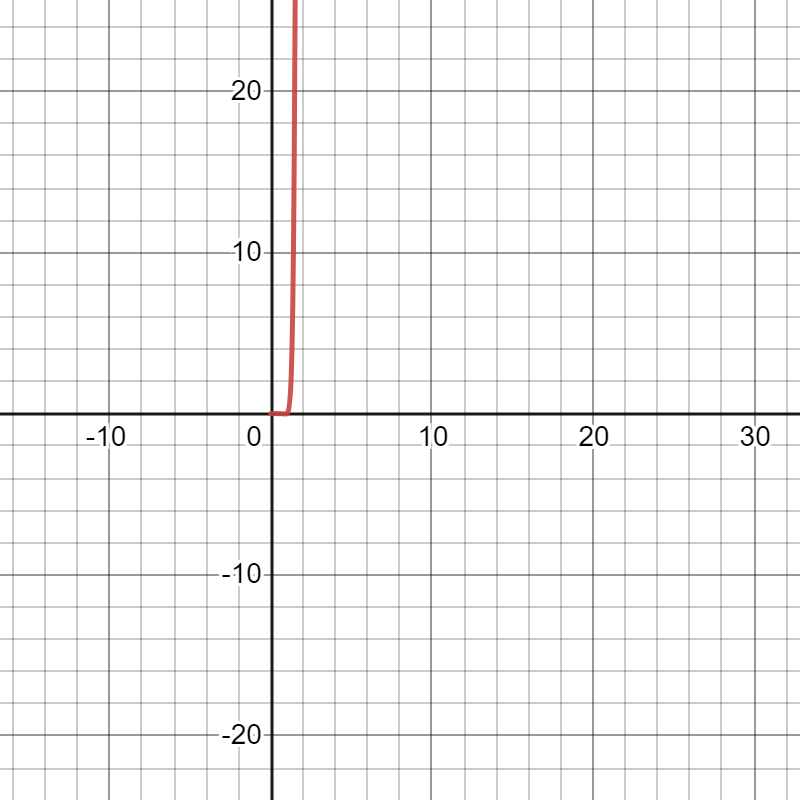
\includegraphics[scale=0.15]{2-10}}}
\caption*{$ \alpha = -10 $}
\end{figure}
\subsubsection{Есть ли значение параметра, при котором легко находится первообразная? Если есть, то найдите её и сделайте вывод о сходимости интеграла}
При $ \alpha = 0 $:\\
\large
$ \int\limits \frac{\ln{x}}{x^{\alpha}}dx = \int\limits \frac{\ln{x}}{x^0}dx = \int\limits \ln{x}dx = u\upsilon - \int\limits ud\upsilon = x\ln{x} - \int\limits x\frac{1}{x}dx = x\ln{x} - x + C = x(\ln{x} - 1) + C $\\
$ f(x) = \lim\limits_{x\to \infty} f(x) = \infty => $ расходится\\\\
\normalsize
При $ \alpha = 1 $:\\
\large
$ \int\limits \frac{\ln{x}}{x}dx = \int\limits udu = \frac{u^2}{2} + C = \frac{\ln^2{x}}{2} + C $\\
\normalsize
При $ \alpha \in Z $: берётся по частям
\subsubsection{Сформулируйте признаки сравнения для определения сходимости несобственных интегралов}
Признаки сравнения:\\
Первый признак сравнения:\\
Если на промежутке $ [a; +\infty) $ непрерывные $ f(x) $ и $ g(x) $ удовлетворяют условию:\\
$ 0 \le f(x) \le g(x) $, то из сходимости интеграла $ \int\limits^{+\infty}_{a} g(x)dx $ следует сходимость интеграла $ \int\limits^{+\infty}_{a} f(x)dx $, а из расходимости интеграла $ \int\limits^{+\infty}_{a} f(x)dx $ следует расходимость интеграла $ \int\limits^{+\infty}_{a} g(x)dx $\\
Второй признак сравнения:\\
Если существует предел $ \lim_{x\to \infty} \frac{f(x)}{g(x)} = k $:\\
$ (0 < k < \infty, f(x) > 0 $ и $ g(x) > 0) $, то интегралы $ \int\limits^{+\infty}_{a} f(x)dx $ и $ \int\limits^{+\infty}_{a} g(x)dx $ одновременно оба сходятся или оба расходятся\\
Но использовать второй признак сравнения нельзя, так как $ k $ является либо нулём, либо бесконечностью, а должно быть каким-то числом. Из-за этого мы должны использовать только первый пункт сравнения, который этим же пунктом и доказывается
\subsubsection{Оцените сверху и снизу трансцендентную функцию (логарифм или арктангенс) для сравнения исходного интеграла с интегралом вида $ \int\limits^b_a \frac{1}{x^{\beta}}dx $. Установите, при каких значениях параметра это сравнение позволяет сделать вывод о сходимости интеграла}
Траснцедентная функция: $ \ln{x} $\\
$ \lim\limits_{x \to +\infty} (\ln{x}) = \infty => $ сверху не ограничена\\
$ \lim\limits_{x \to 1+} (\ln{x}) = 0 $\\
Интеграл для сравнения: $ -\int\limits^{+\infty}_{1} \frac{1}{x^{\beta}}dx $\\
Рассмотрим сходимость интеграла:\\
$ \int\limits^{+\infty}_{1} \ln{x}dx = \lim\limits_{b \to +\infty} \int\limits^{b}_{1} \ln{x}dx = \lim\limits_{b \to +\infty} (\ln{x}x - x |^b_1) = \lim\limits_{b \to +\infty} (\ln{b}b - b + 1) = \lim\limits_{b \to +\infty} (b(\ln{b} - 1) + 1) = \infty => $ интеграл расходится\\
$ \int\limits^{+\infty}_1 \frac{1}{x^{\beta}}dx = \lim\limits_{b \to +\infty} \int\limits^b_1 \frac{1}{x^{\beta}}dx $\\
Рассмотрим возможные значения параметра $\beta$:\\
1. $ \beta < 0 : \lim\limits_{b \to +\infty} \int\limits^b_1 \frac{1}{x^{\beta}}dx = \lim\limits_{b \to +\infty} (\frac{x^{-\beta + 1}}{-\beta + 1} |^b_1) = \lim\limits_{b \to +\infty} (\frac{1}{-\beta+1}*(b^{-\beta+1} - 1)) = \infty $\\
2. $ \beta = 0 : \lim\limits_{b \to +\infty} \int\limits^b_1 \frac{1}{x^{\beta}}dx = \lim\limits_{b \to +\infty} (x |^b_1) = \lim\limits_{b \to +\infty} (b - 1) = \infty $\\
3. $ \beta = 1 : \lim\limits_{b \to +\infty} \int\limits^b_1 \frac{1}{x^{\beta}}dx = \lim\limits_{b \to +\infty} (\ln{|x| |^b_1}) = \lim\limits_{b \to +\infty} (\ln{|b|} - \ln{|1|}) = \infty $\\
4. $ \beta \ge 2 : \lim\limits_{b \to +\infty} \int\limits^b_1 \frac{1}{x^{\beta}}dx = \lim\limits_{b \to +\infty} (\frac{-1}{(\beta - 1) x^{\beta - 1}} |^b_1) = \lim\limits_{b \to +\infty} (\frac{-1}{\beta - 1} * (\frac{1}{b^{\beta - 1}} - 1)) = \frac{1}{\beta - 1} $\\
\small $ x \in [1; +\infty] $\\
\normalsize
$ \ln{x} < \frac{1}{x^\beta} $ , $ \beta \leq -1 $ , $ \ln{x} < \frac{1}{x^{\beta}} $ , $ \ln{x} $ - расх. => $ \frac{1}{x^{\beta}} $ - расх.\\
$ \ln{x} = \frac{1}{x{\beta}} $ \HUGE{X}\\
$ \ln{x} \ge \frac{1}{x^{\beta}} $ - какое $\beta$ не возьми, около $ x = 1 $ $ \frac{1}{x^{\beta}} будет > \ln{x} => $ не выполняется условие сравнения
\subsubsection{Вспомните, как ведёт себя интеграл при значении параметра $ \alpha $, при котором легко находится первообразная. Используйте этот интеграл как эталон для сравнения с интегралом при другом параметре $ \alpha $}
$ a = 0 $\\
$ f_1 = \ln{x} $ - расходящаяся\\
$ a = 1 $\\
$ f_2 = \frac{\ln{x}}{x} $\\
$ \int\limits^{+\infty}_1 \frac{\ln{x}}{x}dx = \lim\limits_{A\to +\infty} \int\limits^A_1 \frac{\ln{x}}{x}dx = \lim\limits_{A\to +\infty} \int\limits^A_1 \ln{x}d(\ln{x}) = \lim\limits_{A\to +\infty} (\frac{\ln^2{x}}{2} |^A_1) = \lim\limits_{A\to +\infty} \frac{\ln^2{A}}{2} = \infty $ - расходящаяся\\
$ f_2 \le f_1 $\\
$ 0 \le \frac{\ln{x}}{x} \le \ln{x} $\\
$ \lim\limits_{x\to +\infty} \frac{f_2}{f_1} = \frac{\ln{x}}{x\ln{x}} = 0 $\\
$ \lim\limits_{x\to +\infty} \frac{f_1}{f_2} = +\infty $
\newpage
\Large
\section{Приложения определенного интеграла}
\normalsize
\subsection{Найти давление воды на поверхность цилиндра диаметром 4м и высотой 6м, если его верхнее основание находится на уровне свободной поверхности воды.}
\begin{figure}[h!]
\fbox{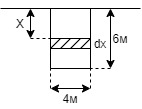
\includegraphics[scale=1]{31}}
\end{figure}
\begin{flushleft}
$\rho$ - плотность жидкости\\
$g$ - гравитационная постоянная, ускорение свободного падения\\
$x$ - глубина погружения\\
$S$ - площадь, на которую действует сила давления\\
$p$ - давление\\
\end{flushleft}
$ p = \rho gxS $ - формула для давления на глубине $x$, действующее на площадь $S$\\
$ dp = \rho gxdS = p_1 $\\
\begin{figure}[h!]
\fbox{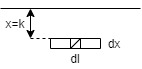
\includegraphics[scale=1]{33}}
\end{figure}\\
$ dS_1 = dx*dl $\\
$ dp_1 = \rho gk*dx*dl $\\
$ p_1 = \int\limits^{2*2\pi}_0 \rho gk*dx*dl = \rho gk*dx \int\limits^{2*2\pi}_0 dl = 4\pi \rho gk*dx $\\
$ p = \int\limits^6_0 4\pi \rho gx*dx = 4\pi \rho g \int\limits^6_0 x*dx = 4\pi \rho g\frac{x^2}{2} |^6_0 = 72\pi \rho g $\\
\small$ g = 9.81 $\\
\normalsize$ 72\pi \rho g \approx 2.21897*10^6$
\newpage
\Large
\section{Приближенные вычисления определенного интеграла}
\normalsize
\subsection{Вычислить значения интеграла $ I^2_0 = \int\limits^2_0 f(x)dx $ по формулам трапеций и парабол при $ h = 1 $, сравнить полученные результаты с точным значением.}
\Large a) $ f(x) = 1 + x $:\\\\
\large\textit{Метод трапеций:}\\
\normalsize
Интервал $ [a; b] = [0; 2], h = 1 $\\
Интервал длины "$h$" $ [0; 1], [1; 2] $\\
$ x_0 = 0 \\ x_1 = 1 \\ x_2 = 2 $\\
$ f(x_0) = 1 \\ f(x_1) = 2 \\ f(x_2) = 3 $\\
1) $ \int\limits^2_0 f(x) \approx \frac{h}{2} (f(x_0) + f(x_1) + f(x_1) + f(x_2)) = \frac{1}{2} (1+4+3) = 4 $\\
2) \large\textit{Метод парабол:}\\
\normalsize
Также разбиваем на отрезки\\
$ x_{2i-2} = x_0 = 0 $\\
$ x_{2i-1} = x_1 = 1 $\\
$ x_{2i} = x_2 = 2 $\\
$ \int\limits^2_0 f(x) \approx \frac{h}{3} (f(0) + 4f(1) + f(2)) = \frac{1}{3} (1 + 8 + 3) = 4 $\\
\small Вывод конечной формулы:
\normalsize
\begin{figure}[h!]
\center{\fbox{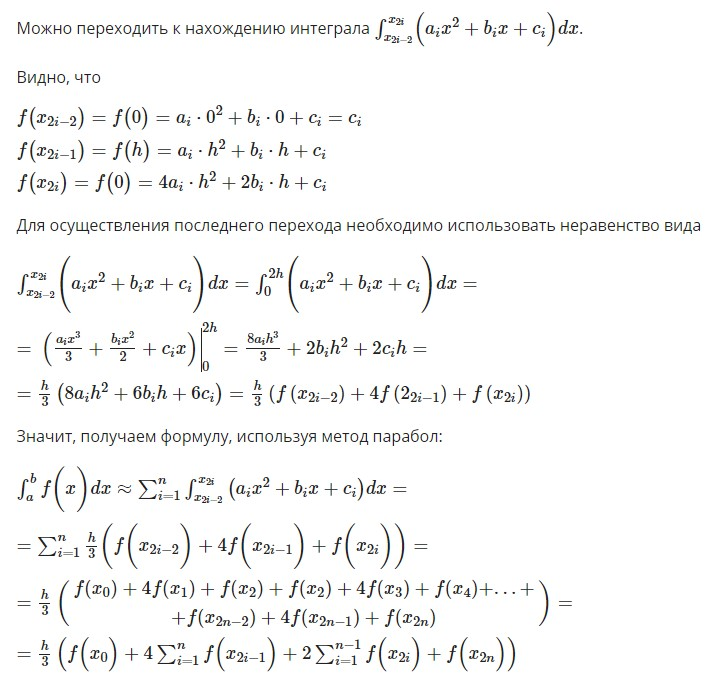
\includegraphics[scale=0.6]{cout4}}}
\end{figure}\\
3) \large\textit{Подсчёт интеграла напрямую:}\\
\normalsize
$ \int\limits^2_0 (x + 1)dx = \frac{x^2}{2} + x |^2_0 = \frac{4}{2} + 2 - 0 = 4 $\\
\newpage
\Large b) $ f(x) = 1 + x^3 $\\
\normalsize
$ x_0 = 0 $\\
$ x_1 = 1 $\\
$ x_2 = 2 $\\\\
Аналогично пункту (а):\\\\
1) $ \int\limits^2_0 \approx \frac{h}{2} (f(x_0) + 2f(x_1) + f(x_2)) = \frac{1}{2} (1+4+9) = 7 $ - большая погрешность, так как много добавленной (добавочной) лишней площади\\
\begin{figure}[h!]
\fbox{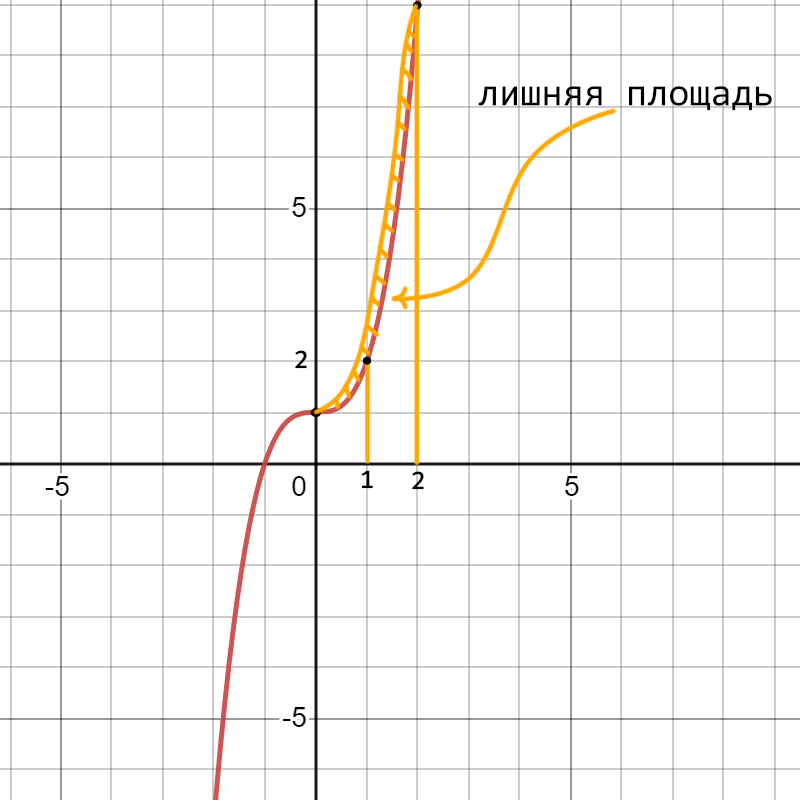
\includegraphics[scale=0.3]{5}}
\end{figure}
\\
2) $ \int\limits^2_0 = \frac{h}{3} (f(0) + 4f(1) + f(2)) = \frac{1}{3} (1+8+9) = 6 $\\
3) $ \int\limits^2_0 = \int\limits^2_0 (x^3 + 1)dx = \frac{x^4}{4} + 4 |^2_0 = \frac{16}{4} + 2 = 6 $\\\\
Вывод:\\
Погрешность вычисления методом трапеций из-за того, что появляется лишняя площадь, а если использовать метод парабол, то мы получаем довольно высокую точность, так как виды функций кубической и обычной парабол похожи.
\end{document}